\subsection{Signed-graph encoding with exact switching symmetry}
\label{sec:conditional-switching16}

We illustrate the construction with a sixteen-qubit encoder that enforces six independent bit-flip symmetries. We consider a temperature-dependent family of signed-graph distributions whose triangle interactions remain invariant under vertex switches. This example demonstrates encoder design and classical access; we do not evaluate learning accuracy for this family.

Sixteen qubits represent the edge signs of a seven-vertex graph. We connect every pair among vertices $0,\ldots,4$, and connect each of vertices $5$ and $6$ to vertices $0,1,2$, as shown in Figure~\ref{fig:switching16-encoder}(a). Each edge bit $x_{ij}$ specifies a sign $s_{ij}=(-1)^{x_{ij}}$. We define the Gibbs family
\begin{equation}
 p_\beta(x)=Z_\beta^{-1}e^{\beta S(x)},\qquad
 S(x)=\sum_{\{i,j,k\}\in\mathcal T}s_{ij}s_{ik}s_{jk},
\end{equation}
where $\beta$ is the inverse temperature, $Z_\beta$ normalizes the distribution, and $\mathcal T$ contains the graph's sixteen triangles. The triangle-balance score $S(x)$ assigns a contribution of $+1$ to each balanced triangle, whose edge signs have positive product, and $-1$ otherwise. Increasing $\beta$ therefore favors configurations with more balanced triangles.

A vertex switch reverses the signs of all edges incident on that vertex. Every triangle contains either zero or two of these edges, so the switch preserves its edge-sign product and hence $p_\beta$. To describe combinations of switches, let $\eta_i\in\{-1,+1\}$ indicate whether vertex $i$ is switched. The combined action replaces $s_{ij}$ by $\eta_i s_{ij}\eta_j$. Switching all seven vertices leaves every edge unchanged, so we fix $\eta_0=1$ to remove duplicate representations. The remaining six choices generate $64$ distinct transformations, including the identity. We denote their edge-bit masks by $G$, so a switch acts as $x\mapsto x\oplus g$ for $g\in G$.

To construct the encoder, we use the six root edges $0i$, with $i=1,\ldots,6$, as a spanning tree. We call the remaining ten edges chords and denote their set by $\mathcal C$. Each chord $ij$ forms a triangle with root edges $0i$ and $0j$. These ten triangles form a cycle basis. In the preceding construction, each column of $C$ is the edge-bit mask of one such triangle, and each latent bit determines whether to include that triangle in the reference configuration. Combining the selected triangles modulo two gives even incidence parity at every vertex.

We prepare this reference state by initializing all sixteen qubits in $\ket{0}$. For each chord $ij$, we apply $R_X(t_\beta)$ to its qubit and two CNOT gates controlled by that qubit, targeting root edges $0i$ and $0j$. On an isolated triangle, these operations prepare $\cos(t_\beta/2)\ket{000}-i\sin(t_\beta/2)\ket{111}$, as illustrated in Figure~\ref{fig:switching16-encoder}(b). In the full graph, the CNOTs combine contributions to shared root edges modulo two. After processing all ten chords, we apply one Hadamard layer to all sixteen qubits to obtain the encoded input.

\begin{figure*}[t]
\centering
\begin{minipage}[c]{0.48\textwidth}
\centering
\textbf{(a)}\par
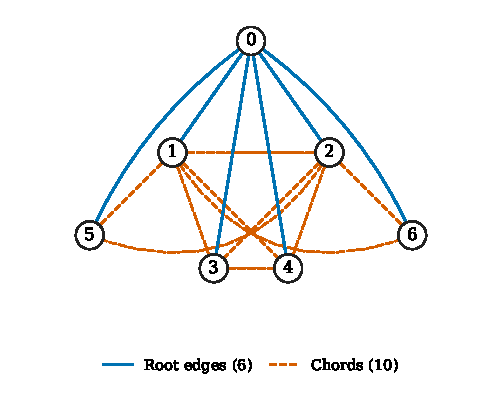
\includegraphics[width=\linewidth]{figures/switching16_graph.pdf}
\end{minipage}\hfill
\begin{minipage}[c]{0.48\textwidth}
\centering
\textbf{(b)}\par
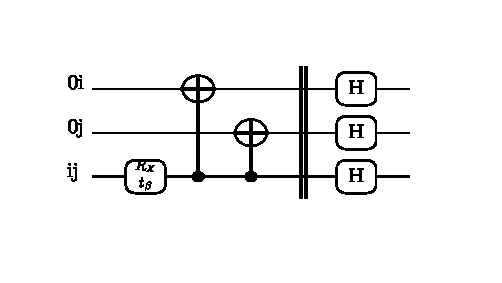
\includegraphics[width=\linewidth]{figures/triangle_motif_draft.pdf}
\end{minipage}
\caption{Signed-graph encoder with six independent switching symmetries. (a) The seven-vertex graph has sixteen edges. Six root edges form a spanning tree, and each of the ten remaining edges forms a fundamental triangle with two root edges. (b) Reference-state preparation on an isolated triangle. A chord rotation $R_X(t_\beta)$ and two CNOTs prepare $\cos(t_\beta/2)\ket{000}-i\sin(t_\beta/2)\ket{111}$ before the displayed Hadamards. For the full encoder, we repeat the rotation--CNOT construction over all ten chords, combining contributions to shared root edges modulo two, then apply one global Hadamard layer. All rotations use $t_\beta=(\pi/2)\tanh(1.5\beta)$.}
\label{fig:switching16-encoder}
\end{figure*}

The encoded input has the form
\begin{align}
 \ket{\phi_\beta}&=\exp\!\left[-\frac{i t_\beta}{2}
 \sum_{(i,j)\in\mathcal C}Z_{0i}Z_{0j}Z_{ij}\right]\ket{+}^{\otimes16},\\
 t_\beta&=\frac{\pi}{2}\tanh(1.5\beta).
\end{align}
We choose this temperature map as a concrete example; the symmetry guarantee does not depend on its form. The diagonal operators leave the computational-basis probabilities uniform, so temperature enters through correlated phases. The shared IQP unitary can convert these phases into condition-dependent output probabilities.

The preparation uses ten rotations, twenty CNOTs and sixteen Hadamards, without ancillary qubits. The state before the Hadamard layer is the reference state used for classical estimation. To sample it, we draw each chord bit independently with probability $\sin^2(t_\beta/2)$ of obtaining one. Each root-edge bit is then the sum, modulo two, of the chord bits incident on its nonzero vertex. The chord bits also determine each supported amplitude through a product of ten rotation coefficients, giving direct amplitude-ratio access. Appendix~\ref{app:switching16} provides the explicit expressions.

Even incidence parity implies that every supported reference configuration has even parity on the edges incident on any switched vertex. The Hadamard layer therefore gives
\begin{equation}
 X_g\ket{\phi_\beta}=\ket{\phi_\beta},
 \qquad g\in G,
\end{equation}
where $X_g$ flips the edge bits selected by $g$. Since the IQP unitary commutes with these operators, the model satisfies
\begin{equation}
 q_{\boldsymbol\theta}(x\mid\beta)
 =q_{\boldsymbol\theta}(x\oplus g\mid\beta),
 \qquad g\in G,
\end{equation}
for every condition and parameter vector. Thus, the encoder enforces all six independent switching symmetries while retaining classical sampling and amplitude-ratio access, without restricting the learned IQP phases.
